\documentclass{article}

% Language setting
% Replace `english' with e.g. `spanish' to change the document language
\usepackage[english]{babel}

% Set page size and margins
% Replace `letterpaper' with`a4paper' for UK/EU standard size
\usepackage[letterpaper,top=2cm,bottom=2cm,left=3cm,right=3cm,marginparwidth=1.75cm]{geometry}

% Useful packages
\usepackage{amsmath}
\usepackage{ccfonts}
% \usepackage{fontspec}
\usepackage{graphicx}
\usepackage[colorlinks=true, allcolors=blue]{hyperref}
\usepackage{xcolor}

% \setmainfont{CMU Concrete}
\newcommand{\rdho}{\textcolor{magenta}{\partial}}
\newcommand{\cdho}{\textcolor{orange}{\partial}}


\title{Backpropagation Derivation}
\author{You}

\begin{document}
\author{Pradeep Ranganathan}
\maketitle

In this document, we derive back-prop equations for a simple 2-hidden-layer neural-net and show how we can take advantage of repeated expressions in partial derivative evaluation to efficiently compute the gradient via back-propagation.

\section{The Model}
\begin{center}
    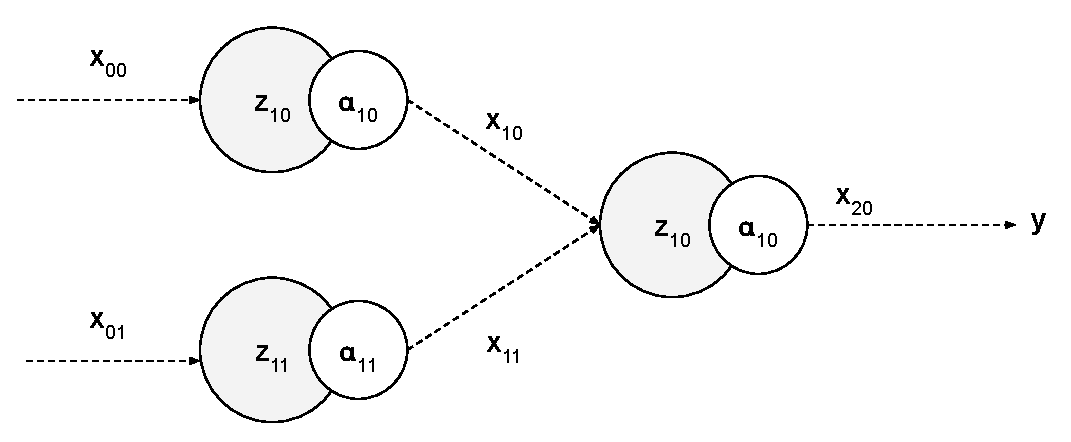
\includegraphics[scale=0.64]{2-Layer-Neural-Net.pdf}
\end{center}
Each neural unit computes a linear function of its input \(z = wx + b\) and then sends the linear output through a non-linear activation function \(\alpha(\cdot)\). We assume that all neural units use the same activation function, \(\alpha\), as is common in practice.
Hence for the first layer that operates on the inputs, \(x_{10}\) and \(x_{11}\), we have:
\begin{align*}
    z_{10} &= w_{10}x_{00} + b_{10} \\
    x_{10} &= \alpha(z_{10}) \\
    z_{11} &= w_{11}x_{01} + b_{11} \\
    x_{11} &= \alpha(z_{11}) \\
\intertext{For the second layer, the neural unit operates on a vector of inputs, \(\mathbf{x}_{1} = \left[x_{10}\ x_{11}\right]^{\top} \). For computation of the back-prop equations we expand the vector linear operation into it constituent scalar parts:}
    z_{20} &= \mathbf{w}_{20}^{\top}\mathbf{x}_{1} + \mathbf{b}_{20} \\
    z_{20} &= (w_{20}^{[0]}x_{10} + b_{20}^{[0]}) + (w_{20}^{[1]}x_{11} + b_{20}^{[1]}) \\
    x_{20} &= \alpha(z_{20}) \\
\intertext{Finally, the output, \(y\), is the output of the last neuron:}
    y &= x_{20}
\end{align*}

\section{Back-prop equations}
\subsection{Partial derivative w.r.t \(w_{10}\)}
\label{ssec-pd-w10}
\text{Using \(\rdho\) to denote the operator \(\frac{\partial}{\partial w_{10}}\)}:
\begin{align*}
    \frac{\partial}{\partial w_{10}} y \
        &= \rdho x_{20} \\
        &= \rdho \alpha(z_{20}) \\
        &= \alpha'(z_{20}) \cdot \rdho z_{20} \\
        &= \alpha'(z_{20}) \cdot \rdho \left\{ (w_{20}^{[0]}x_{10} + b_{20}^{[0]}) + (w_{20}^{[1]}x_{10} + b_{20}^{[1]}) \right\} \\
        &= \alpha'(z_{20}) \cdot \left\{ w_{20}^{[0]}\rdho x_{10} + w_{20}^{[1]} \rdho x_{11} \right\} \\
        &= \alpha'(z_{20}) \cdot \left\{ w_{20}^{[0]}\rdho \alpha(z_{10}) + w_{20}^{[1]} \rdho \alpha(z_{11}) \right\} \\
        &= \alpha'(z_{20}) \cdot \left\{ w_{20}^{[0]} \alpha'(z_{10}) \rdho(w_{10}x_{00} + b_{10}) + w_{20}^{[1]} \alpha'(z_{11}) \rdho(w_{11}x_{01} + b_{11}) \right\} \\
        &= \alpha'(z_{20}) \cdot \left\{ w_{20}^{[0]} \alpha'(z_{10})x_{00}\rdho w_{10} + 0 \right\} \\
        &= \alpha'(z_{20}) \cdot w_{20}^{[0]} \alpha'(z_{10})x_{00}
\end{align*}

\subsection{Partial derivative w.r.t \(w_{11}\)}
\label{ssec-pd-w11}
\text{Using \(\cdho\) to denote the operator \(\frac{\partial}{\partial w_{11}}\)}:
\begin{align*}
    \frac{\partial}{\partial w_{11}} y \
        &= \cdho x_{20} \\
        &= \cdho \alpha(z_{20}) \\
        &= \alpha'(z_{20}) \cdot \cdho z_{20} \\
        &= \alpha'(z_{20}) \cdot \cdho \left\{ (w_{20}^{[0]}x_{10} + b_{20}^{[0]}) + (w_{20}^{[1]}x_{10} + b_{20}^{[1]}) \right\} \\
        &= \alpha'(z_{20}) \cdot \left\{ w_{20}^{[0]}\cdho x_{10} + w_{20}^{[1]} \cdho x_{11} \right\} \\
        &= \alpha'(z_{20}) \cdot \left\{ w_{20}^{[0]}\cdho \alpha(z_{10}) + w_{20}^{[1]} \cdho \alpha(z_{11}) \right\} \\
        &= \alpha'(z_{20}) \cdot \left\{ w_{20}^{[0]} \alpha'(z_{10}) \cdho(w_{10}x_{00} + b_{10}) + w_{20}^{[1]} \alpha'(z_{11}) \cdho(w_{11}x_{01} + b_{11}) \right\} \\
        &= \alpha'(z_{20}) \cdot \left\{ 0 + w_{20}^{[1]} \alpha'(z_{11}) \cdho(w_{11}x_{01} + b_{11}) \right\} \\
        &= \alpha'(z_{20}) \cdot w_{20}^{[1]} \alpha'(z_{11})x_{01}
\end{align*}

\subsection{Other partial derivatives}
The other partial derivatives can be computed in a similar manner. We summarize all partial derivatives w.r.t the parameters of the neural-net below:
\begin{align*}
    \frac{\partial}{\partial b_{20}^{[0]}} y \
        &= \alpha'(z_{20}) \\
    \frac{\partial}{\partial b_{20}^{[1]}} y \
        &= \alpha'(z_{20}) \\
    \frac{\partial}{\partial w_{20}^{[0]}} y \
        &= \alpha'(z_{20}) \cdot x_{10} \\
    \frac{\partial}{\partial w_{20}^{[1]}} y \
        &= \alpha'(z_{20}) \cdot x_{11} \\
    \frac{\partial}{\partial b_{10}} y \
        &= \alpha'(z_{20}) \cdot w_{20}^{[0]} \alpha'(z_{10}) \\
    \frac{\partial}{\partial w_{10}} y \
        &= \alpha'(z_{20}) \cdot w_{20}^{[1]} \alpha'(z_{10})x_{00} & \text{(derived in \ref{ssec-pd-w10})} \\
    \frac{\partial}{\partial b_{11}} y \
        &= \alpha'(z_{20}) \cdot w_{20}^{[1]} \alpha'(z_{11}) \\
    \frac{\partial}{\partial w_{11}} y \
        &= \alpha'(z_{20}) \cdot w_{20}^{[1]} \alpha'(z_{11})x_{01} & \text{(derived in \ref{ssec-pd-w11})}
\end{align*}

\section{Efficient back-prop}
After examining the above expressions it should be apparent that the sub-expressions \(\alpha'(z_{20})\), \(\alpha'(z_{20}) \cdot w_{20}^{[0]} \) and \(\alpha'(z_{20}) \cdot w_{20}^{[1]} \) are shared amongst different sub-sets of partial derivative expressions.

By collecting common sub-expressions from the partial derivative expressions and creating an directed acyclic graph using {\em is-a-subexpression-of} relations, it is possible to produce a series of compounding computations that evaluate each partial derivative with a constant amount of computation on top of existing expressions. This lead-us to a back-to-front evaluation strategy where sub-expressions are computed and reused, starting from the last-layer to the first and hence the term {\em back-propagation of errors}.

\end{document}